\section{Methodology}\label{methodology}

Since we wish to analyze software testing literature, we collect data (both
correct and incorrect) from a wide variety of relevant documents, focusing on
test approaches and supporting information. This results in a big messy
glossary of software approaches, some glossaries of supplementary terms, and a
list of flaws. To ensure this data can be analyzed and expanded thoroughly and
consistently, we need a process that can be repeated for future developments in
the field of software testing, or by independent researchers seeking to verify
our work. Our methodology for documenting the current (messy) state of software
testing terminology consists of:

\input{build/methodOverview}

\subsection{Sources}\label{sources}
As there is no single authoritative source on software testing terminology,
we need to look at many sources to observe how this terminology is used in
practice. Since we are particularly interested in software engineering, we
start from the vocabulary document for systems and software engineering%
\qtodo{Better name for this?}
\citep{IEEE2017} and two versions of the \acf{swebok}---the newest
one \citep{SWEBOK2014} and one submitted for public review\footnote{
    \refHelper \citep{SWEBOK2024} has been published since we investigated
    these sources; if time permits, we will revisit this published version.
} \citep{SWEBOK2024}. To gather further sources, we then use a version of
``snowball sampling'',
which ``is commonly used to locate hidden populations \dots{} [via] referrals
from initially sampled respondents to other persons'' \citep{Johnson2014}. We
apply this concept to ``referrals'' between sources. \addTextEx{}

For ease of discussion and analysis, we group the complete set of sources into
``tiers'' based on their format, method of publication, and our heuristic of
credibility (defined in \Cref{cred}). In order of descending credibility, we
define the following tiers:
\begin{enumerate}
    \item established standards (\Cref{stds}),
    \item terminology collections (\Cref{metas}),
    \item textbooks (\Cref{texts}), and
    \item papers and other documents (\Cref{papers}).
\end{enumerate}
We provide a summary of how many sources comprise each tier in
\Cref{fig:sourceSummary}\ifnotpaper\ and list all sources in each tier
    in \Cref{app-src-tiers}\fi. The ``papers'' tier is quite large since we
often ``snowball'' on terminology itself when a term requires more
investigation (e.g., its definition is missing or unclear). This includes
performing a miniature literature review on this subset to ``fill in'' missing
information (see \Cref{undef-terms}) and potentially fully investigating these
additional sources, as opposed to just the original subset of interest,
based on their credibility and how much extra information they provide.
We use standards the second most frequently due to their high credibility and
broad scope; for example, the glossary portion of \citet{IEEE2017} has 514
pages! Using these standards allows us to record many test approaches in a
similar context from a source that is widely used and well-respected.

% Only top or bottom to comply with IEEE guidelines
\begin{figure}[bt!]
    \centering
    \begin{tikzpicture}
        \pie[sum=auto, after number=, text=legend, thick,
            scale=\ifnotpaper0.7\else0.5\fi,
            every label/.style={align=left, scale=0.7}]
        {\stdSources{3}/\stds{},
            \metaSources{3}/\metas{},
            \textSources{3}/\texts{},
            \paperSources{3}/\papers{}}
    \end{tikzpicture}
    \caption{Summary of how many sources comprise each source tier.}
    \label{fig:sourceSummary}
\end{figure}

\subsubsection{\stdSources{1}}\label{stds}
% Colored \textcolor{green}{green}

These are documents written for the field of software engineering by reputable
standards bodies, namely ISO, the \acf{iec}, and IEEE. Their purpose is to
``encourage the use of systems and software engineering standards'' and
``collect and standardize terminology'' by ``provid[ing] definitions that are
rigorous, uncomplicated, and understandable by all concerned''
\citep[p.~viii]{IEEE2017} ``that can be used by any organization when
performing any form of software testing''
\ifnotpaper(\fi\citeyear[p.~vii]{IEEE2022}\ifnotpaper; similar in
\citeyear[p.~ix]{IEEE2016})\fi. For these reasons, they
are the most credible sources. However, this does not imply perfection, as we
identify \stdFlawMnfstBrkdwn{13} % is (should be!) equal to \stdFlawDmnBrkdwn{15}
flaws within these standards (see \Cref{tab:flawMnfsts,tab:flawDmns})!
Only standards for software development and testing are in scope for
this research (see \Cref{scope-overview}).
% For example, ``the purpose of the
% ISO/IEC/IEEE 29119 series is to define an internationally agreed set of
% standards for software testing that can be used by any organization when
% performing any form of software testing''
% \ifnotpaper(\fi\citeyear[p.~vii]{IEEE2022}\ifnotpaper; similar in
% \citeyear[p.~ix]{IEEE2016})\fi.

\subsubsection{\metaSources{1}}\label{metas}
% Colored \textcolor{blue}{blue}

These are collections of software testing terminology built up from multiple
sources, such as the established standards outlined in \Cref{stds}. For
example, the \acs{swebok} is ``proposed as a
suitable foundation for government licensing, for the regulation of software
engineers, and for the development of university curricula in software
engineering'' \citep[p.~xix]{KanerEtAl2011}. Even though it is ``published by
the IEEE Computer Society'', it ``reflects the current state of generally
accepted, consensus-driven knowledge derived from the interaction between
software engineering theory and practice'' \citep{AboutSWEBOK}. Due to this
combination of IEEE standards and state-of-the-practice observations, we
designate it as a collection of terminology as opposed to an established
standard. Collections such as this are often written by a large
organization, such as the \acf{istqb}, but not always. \ifnotpaper \else
    \citeauthor{Firesmith2015} \fi \citet{Firesmith2015}'s taxonomy presents
relations between many test approaches and \ifnotpaper \else
    \citeauthor{DoğanEtAl2014} \fi \citet{DoğanEtAl2014}'s literature
review cites many sources from which we can ``snowball'' if desired
(see \Cref{sources}), so we include them in this tier as well.

\subsubsection{\textSources{1}}\label{texts}
% Colored \textcolor{Maroon}{maroon}

We consider textbooks to be more credible than papers (see \Cref{papers})
because they are widely used as resources for teaching software engineering and
industry frequently uses them as guides. Although textbooks have smaller sets of
authors, they follow a formal review process before publication. Textbooks used
at McMaster University \citep{Patton2006,PetersAndPedrycz2000,vanVliet2000}
served as the original (albeit ad hoc and arbitrary) starting point of this
research, and we investigate other books as they arise. \addTextEx{}

\subsubsection{\paperSources{1}}\label{papers}
% Colored black

The remaining documents all have much smaller sets of authors and are much less
widespread than those in higher source tiers. While most of these are journal
articles and conference papers, we also include the following document types.
Some of these are not peer-reviewed works but are still useful for
observing how terms are used in practice\thesisissueref{89}:

\begin{itemize}
    \item Report \citep{Kam2008,Gerrard2000a,Gerrard2000b}
    \item Thesis \citep{Bas2024}
          % \item A less-formal classification \citep{KuļešovsEtAl2013}
    \item Website \citep{LambdaTest2024,Pandey2023}
    \item Booklet \citep{SPICE2022}
    \item \ifnotpaper \else ChatGPT \fi \citet{ChatGPT2024} (with its claims
          supported by \citet{RusEtAl2008})
\end{itemize}

\subsection{Identifying Relevant Terms}\label{ident-terms}
Before we can consistently track software testing terminology used in the
literature, we must first determine what to record. We use heuristics to guide
this process to increase confidence that we identify all relevant terms, paying
special attention to the following when investigating a new source:
\begin{itemize}
    \item glossaries, taxonomies, hierarchies, and lists of terms,
    \item testing-related terms (e.g., terms containing ``test(ing)'',
          \ifnotpaper ``review(s)'', ``audit(s)'', ``attack(s)''%
              \thesisissueref{55}, \fi ``validation'', or ``verification''),
    \item terms that had emerged as part of already-discovered
          test approaches, \emph{especially} those that were ambiguous
          or prompted further discussion (e.g., terms containing
          ``performance'', ``recovery'', ``component'', ``bottom-up'',
          \ifnotpaper ``boundary'', \fi or ``configuration''), and
    \item terms that imply test approaches\ifnotpaper\footnote{
                  Since these methods for deriving test approaches only arose
                  as research progressed, some examples would have been missed
                  during the first pass(es) of resources investigated earlier
                  in the process. While reiterating over them would be ideal,
                  this may not be possible due to time constraints.
              }% (see \Cref{derived-tests})
          \fi, including:
          \newcommand\derivTest[2]{#1 that may imply \ifnotpaper related \fi test #2}
          \begin{itemize}
              \item \derivTest{coverage metrics}{techniques},
              \item \phantomsection{}\label{qual-types}
                    \derivTest{software qualities}{types}, and
              \item \phantomsection{}\label{req-apps}
                    \derivTest{\ifnotpaper software \fi requirements}{approaches}.
          \end{itemize}
\end{itemize}
We apply these heuristics to the entirety of most investigated sources,
especially established standards (see \Cref{stds}). However, we only partially
investigate some sources, such as those chosen for a specific area of
interest or based on a test approach that was determined to be out-of-scope.
These include the following sources as described in \Cref{undef-terms}:
\citet{ISO2022,ISO2015,Dominguez-PumarEtAl2020,PierreEtAl2017,
    TrudnowskiEtAl2017,YuEtAl2011,Tsui2007,Goralski1999}.
During the first pass of data collection, we investigate and record all
approaches to software testing. Some of these approaches are less
applicable to our original motivation of test case automation \ifnotpaper
    (such as static testing; see \Cref{static-test}\thesisissueref{39}) \fi or
are quite broad\ifnotpaper\ (such as attacks%
    %; see \Cref{attacks}
    \thesisissueref{55})\fi, so we will omit them during future analysis.

\subsection{Recording Relevant Terms}\label{record-terms}

\ifnotpaper
    % Based on https://www.overleaf.com/learn/latex/LaTeX_Graphics_using_TikZ%3A_A_Tutorial_for_Beginners_(Part_3)%E2%80%94Creating_Flowcharts

\tikzstyle{startend} = [rectangle, rounded corners,
minimum width=3cm,
minimum height=1cm,
text centered,
text width=3cm,
draw=black,
fill=red!30]

\tikzstyle{io} = [trapezium,
trapezium stretches=true, % A later addition
trapezium left angle=70,
trapezium right angle=110,
minimum width=3cm,
minimum height=1cm,
text centered,
text width=3cm,
draw=black, fill=blue!30]

\tikzstyle{process} = [rectangle,
minimum width=3cm,
minimum height=1cm,
text centered,
text width=4.25cm,
draw=black,
fill=orange!30]

% Hacky but I can't think of a better way to do this
\tikzstyle{decisionL} = [diamond,
aspect=1.75,
minimum width=0.25cm,
minimum height=0.25cm,
text centered,
text width=3cm,
draw=black,
fill=green!30]

\tikzstyle{decisionS} = [diamond,
aspect=1.75,
minimum width=0.25cm,
minimum height=0.25cm,
text centered,
text width=2cm,
draw=black,
fill=green!30]

\tikzstyle{arrow} = [thick,->,>=stealth]

\begin{figure}
    \adjustbox{scale=0.89}{
        \begin{tikzpicture}[node distance=2cm]

            \node (start)   [startend, xshift=-5cm] {Start};
            \node (ident)   [io, right of=start, xshift=3.5cm] {Test Approach Identified};
            \node (present) [decisionS, right of=ident, xshift=3cm] {Present in Glossary?};

            \node (newrow) [process, below of=present, yshift=-0.5cm] {Create New Row in Glossary};
            \node (newapp) [process, below of=newrow] {Record Approach Name and Category as ``Approach''};

            \node (catapp)   [decisionL, below of=start,  yshift=-0.5cm] {Present Category is ``Approach''?};
            \node (catgiven) [decisionS, below of=ident,  yshift=-0.5cm] {Category Given?};
            \node (catmatch) [decisionL, below of=catapp, yshift=-2.5cm] {Given Category Matches Present Category?};

            \node (catreplace) [process, below of=catgiven,   yshift=-1.5cm, xshift=-0.5cm] {Replace ``Approach'' with Given Category};
            \node (catmatches) [process, below of=catmatch,   yshift=-1cm] {Add Citation for Category};
            \node (catnomatch) [process, below of=catreplace, yshift=-1cm] {Add Given Category};

            \node (data)        [io,        below of=newapp,      yshift=-3.5cm] {Additional Approach Data Identified};
            \node (datagiven)   [decisionL, below of=catnomatch,  yshift=-1.5cm] {Given Data Matches Present Data?};
            \node (datanomatch)   [process, below of=datagiven,   yshift=-1.5cm] {Add Given Data and Document as Flaw (as applicable)};
            \node (datamatch)     [process, left of=datanomatch,  xshift=-3cm]   {Add Citation for Data};
            \node (datasomematch) [process, right of=datanomatch, xshift=3cm]    {Merge with Present Data};

            \node (end) [startend, below of=datanomatch] {End};

            \draw [arrow] (start) -- (ident);
            \draw [arrow] (ident) -- (present);
            \draw [arrow] (present) -- node[anchor=south] {yes} (catgiven);
            \draw [arrow] (present) -- node[anchor=east]  {no}  (newrow);
            \draw [arrow] (newrow) -- (newapp);
            \draw [arrow] (newapp.west) -- (catgiven);

            \draw [arrow] (catgiven) -- node[anchor=south] {yes} (catapp);
            \draw [arrow] (catapp)   -- node[anchor=south] {\enspace yes} (catreplace);
            \draw [arrow] (catapp)   -- node[anchor=east]  {no}  (catmatch);
            \draw [arrow] (catmatch) -- node[anchor=east]  {yes} (catmatches);
            \draw [arrow] (catmatch) -- node[anchor=south] {no}  (catnomatch);

            \draw [arrow] (catgiven) -- node[anchor=west] {no} (data);
            \draw [arrow] (catmatches) -- (data);
            \draw [arrow] (catnomatch) -- (data);
            \draw [arrow] (catreplace) -- (data);

            \draw [arrow] (data) -- (datagiven);
            \draw [arrow] (datagiven) -- node[anchor=east] {yes\enspace} (datamatch);
            \draw [arrow] (datagiven) -- node[anchor=east] {no} (datanomatch);
            \draw [arrow] (datagiven) -- node[anchor=west] {\quad somewhat} (datasomematch);

            \draw [arrow] (datamatch)     -- (end);
            \draw [arrow] (datanomatch)   -- (end);
            \draw [arrow] (datasomematch) -- (end);

        \end{tikzpicture}
    }
    \caption{Procedure for recording test approaches in our glossary; ``Present''
        refers to data already in our glossary, while ``Given'' refers to data
        that appears in the source being investigated.}\label{fig:recAppFlowchart}
\end{figure}
\fi

Once we have identified which terms from the literature are relevant, we can
then track them consistently. We do this by building glossaries, mainly
focusing on the one most central to our research---\ourApproachGlossary{}---where
we record all test approaches we identify in the literature. We give each test
approach its own row where we record its name and any given \approachFields{}
(along with any other notes, such as questions, prerequisites, and other
resources to investigate) following the procedure in \Cref{fig:recAppFlowchart}.
Note that only the name and category fields are required; all other fields
may be left blank, although a lack of definition indicates that the approach
should be investigated further to see if its inclusion is meaningful (see
\Cref{undef-terms}). When recording flawed data, we record it in our glossary as
dubious information (see \Cref{\ifnotpaper imp-case-four\else imp-case-three\fi})
and/or in a separate document if it is clearly flawed (see \Cref{flaw-def}).
% If no category is given, the ``approach'' category is assigned
% (with no accompanying citation) as a ``catch-all'' category. 
% Any additional information from other sources is added to
% or merged with the existing information in our glossary where appropriate.
% This includes the generic ``approach'' category being replaced with a more
% specific one, an additional synonym being mentioned, or another source
% describing an already-documented parent-child relation. If any new information
% does not agree with existing information or indicates a potential flaw, …
% When new information does not conflict with existing information, we either
% keep the clearest and most concise version or merge them to paint a more
% complete picture.

\begin{figure}[bt!]
    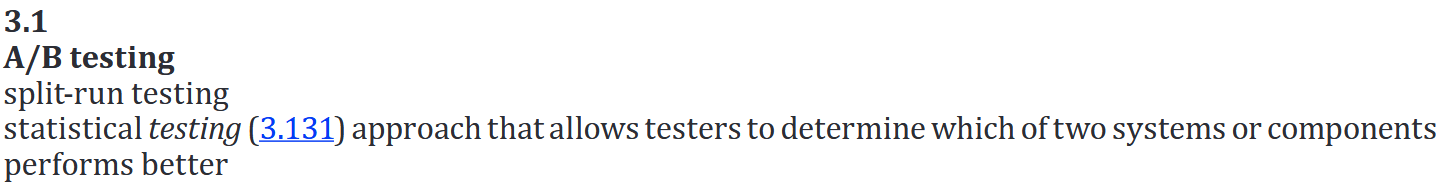
\includegraphics[width=\linewidth]{assets/images/a-b testing.png}
    \caption{\refHelper \citet[p.~1]{IEEE2022}'s glossary entry for
        ``A/B testing''.}\label{fig:IEEE-A-B-Testing}
\end{figure}

For example, \citet[p.~1, 36]{IEEE2022} \multiAuthHelper{define} ``A/B testing''
as shown in \Cref{fig:IEEE-A-B-Testing}. Since we do not yet have a row for
``A/B testing'' in \ourApproachGlossary{}, we apply our procedure as follows:%
\qtodo{Should glossary headers be capitalized?}
\begin{enumerate}
    \item Create a new row with the name ``A/B testing'' and the category
          ``Approach'' (see \Cref{cats-def}).
    \item Record the synonym ``Split-Run Testing'' (see \Cref{syn-rels}).
    \item Record the parent ``Statistical Testing'' (see \Cref{par-chd-rels}).%
          \qtodo{Are these references helpful or distracting?}
    \item Record the definition ``Testing `that allows testers to determine
          which of two systems or components performs better'\,''; note that
          we abstract away information that we have previously captured (i.e.,
          its synonym and parent).
\end{enumerate}
Note that we accompany all of these entries (excluding its name) with the
citation ``\citep[pp.~1, 36]{IEEE2022}''. This document provides more
information which we capture as follows:
\begin{enumerate}
    \item Record the note ``It `can be time-consuming, although tools can be
          used to support it', `is a means of solving the test oracle problem
          by using the existing system as a partial oracle', and is `not a test
          case generation technique as test inputs are not generated'\,''
          \citetext{p.~36}.
    \item Replace the category of ``Approach'' with the more specific
          ``Practice'' \citetext{Fig.~2} (see \Cref{cats-def}); note that this
          is consistent with the exclusion of ``Technique'' as a possible
          category for this approach from page~36.
\end{enumerate}
As we investigate other sources, we learn more about this approach. \ifnotpaper
\else \citeauthor{Firesmith2015} \fi \citet[p.~58]{Firesmith2015} includes it
in his taxonomy as shown in \Cref{fig:Firesmith-A-B-Testing}. We add to our
entry for ``A/B Testing'' as follows:

\begin{minipage}{0.45\linewidth}
    \vspace{0.5cm}
    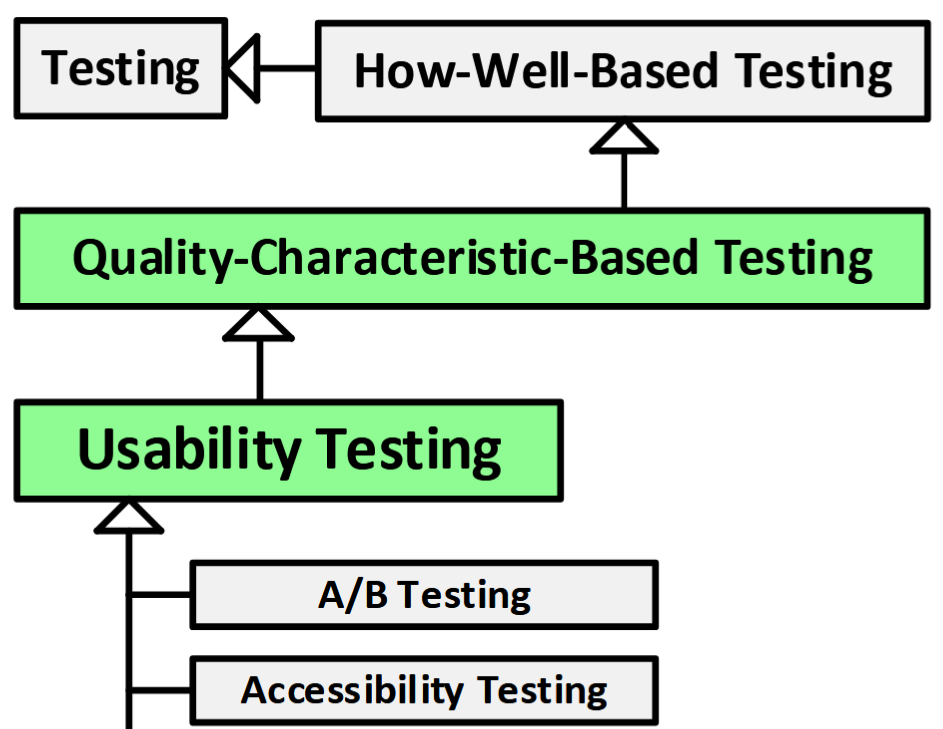
\includegraphics[width=\linewidth]{assets/images/a-b testing 2.png}
    \captionof{figure}{A/B testing's inclusion in \ifnotpaper \else
            \citeauthor{Firesmith2015} \fi \citet[p.~58]{Firesmith2015}'s
        taxonomy.}\label{fig:Firesmith-A-B-Testing}
    \vspace{0.5cm}
\end{minipage}
\begin{minipage}{\ifnotpaper 0.53\else 0.5\fi\linewidth}
    \begin{enumerate}
        \item Add the parent ``Usability Testing''.
        \item Since usability testing is a test type \ifnotpaper
                  (\citealp[pp.~22, 26\=/27]{IEEE2022};
                  \citeyear[pp.~7, 40, Tab.~A.1]{IEEE2021};
                  implied by its quality; \citealp[p.~53]{Firesmith2015})\else
                  \cite[pp.~22, 26\=/27]{IEEE2022},
                  \cite[pp.~7, 40, Tab.~A.1]{IEEE2021}\fi, add the category
              ``Type'' with the citation ``(inferred from usability testing)''%
              \ifnotpaper\ (see \Cref{infers})\fi.
    \end{enumerate}
\end{minipage}\qtodo{Is my justification for inferring ``Type'' sufficient?}
This second change violates our assumption that categories are
orthogonal\ifnotpaper\ (see \Cref{orth-approach})\fi, so we consider this to be
an inferred flaw \ifnotpaper (defined in \Cref{infers}) \fi that we
automatically detect and document \ifnotpaper (see \Cref{auto-flaw-analysis,%
        tab:infMultiCats}, respectively). This results in the corresponding row
    in \Cref{tab:approachGlossaryExcerpt} although we exclude the ``Notes''
    column for brevity\else (details omitted for brevity)\fi.

\phantomsection{}\label{qual-supp-procedure}
We use similar procedures to track software qualities and supplementary
terminology (either shared by multiple approaches or too complicated to explain
inline) in separate glossaries with a similar format. This includes recording
the name, definition, and synonym(s) of these terms, as well as any precedence
for a related test type for a given software quality. For example, analyzability%
\footnote{This may be spelled ``analyzability'' \citep[p.~18]{IEEE2017} or
    ``analysability'' \citep{ISO_IEC2023a}; since this is a dialectal
    difference, we do not count this as a label flaw (described in
    \Cref{label-flaw-def}).}, modifiability, modularity, reusability, and
testability are all subqualities of maintainability \ifnotpaper
    (\citealp{ISO_IEC2023a}; \citealp[Tab.~A.1]{IEEE2021};
    \citealp[p.~7\=/10]{SWEBOK2024}) \else
    \cite[p.~7\=/10]{SWEBOK2024}, \cite[Tab.~A.1]{IEEE2021},
    \cite{ISO_IEC2023a} \fi which has an associated test type
\ifnotpaper
    (\citealp[pp.~5, 22]{IEEE2022}; \citeyear[p.~38, Tab.~A.1]{IEEE2021})\else
    \cite[pp.~5, 22]{IEEE2022}, \cite[p.~38, Tab.~A.1]{IEEE2021}\fi. This sets
a ``precedent'' for each of these subqualities having its own associated test
type (e.g., reusability testing). \ifnotpaper
    Sometimes, the literature provides a relation between qualities where at
    least one of them does not have an explicit approach associated with it
    (although it may be inferred). We record this information regardless, since
    it may become relevant if an associated test type emerges as alluded to
    \hyperref[qual-types]{earlier}. For example, \citet{ISO_IEC2023a} provides
    relations involving dependability and modifiability, but only in terms of
    them as qualities, not types of testing. We record these relations in case
    an associated test type is explicitly named by the literature, which would
    inherit these relations. \fi

% \subsubsection{Derived Test Approaches}\label{derived-tests}

% Throughout this research, we noticed many groups of test approaches that arise
% from some underlying area of software (testing) knowledge. The legitimacy of
% extrapolating new test approaches from these knowledge domains is heavily
% implied by the literature, but not explicitly stated as a general rule. Regardless,
% since the field of software is ever-evolving, it is crucial to be able to
% adapt to, talk about, and understand new developments in software testing.
% Bases for defining new test approaches suggested by the literature include
% coverage metrics, software qualities, and attacks. These are meaningful
% enough to merit analysis and are therefore in scope. Requirements may also
% imply related test approaches, but this mainly results in test approaches
% that would be out of scope. \ifnotpaper Other test approaches found in the
%     literature are derived from programming languages or other orthogonal test
%     approaches, but these are out of scope as this information is better
%     captured by other approaches (see \Cref{lang-test,orth-test}, respectively).

%     \paragraph{Coverage-driven Techniques}\label{cov-test}

%     Test techniques are able to ``identify test coverage items \dots{} and
%     derive corresponding test cases''
%     \ifnotpaper
%         (\citealp[p.~11]{IEEE2022}; similar in \citeyear[p.~467]{IEEE2017})
%     \else
%         \cite[p.~11]{IEEE2022} (similar in \cite[p.~467]{IEEE2017})
%     \fi
%     in a ``systematic'' way
%     \citeyearpar[p.~464]{IEEE2017}.
%     \ifnotpaper
%         This allows for ``the coverage achieved by a specific test design
%         technique'' to be calculated as a percentage of ``the number of test
%         coverage items covered by executed test cases'' \citeyearpar[p.~30]{IEEE2021}.
%         %     ``Coverage levels can range
%         %     from 0\% to 100\%'' and may or may not include ``infeasible'' test coverage
%         %     items, which are ``not \dots{} executable or [are] impossible to be covered by a
%         %     test case'' \citetext{p.~30}. Perhaps more interestingly, the further
%         %     implication is
%         % \else
%         %     This means
%     \fi % that
%     Therefore, a given coverage metric implies a test approach aimed to
%     maximize it. For example, path testing ``aims to execute all entry-to-exit
%     control flow paths in a \acs{sut}'s control flow graph'' \citep[p.~5-13]{SWEBOK2024},
%     thus maximizing the path coverage
%     \ifnotpaper
%         \citep[see][Fig.~1\thesisissueref{63}]{SharmaEtAl2021}\else
%         (see \cite[Fig.~1]{SharmaEtAl2021}\thesisissueref{63})\fi.

%     \paragraph{Quality-driven Types}\label{qual-test}

%     Since test types are ``focused on specific quality characteristics''
%     \ifnotpaper
%         (\citealp[p.~15]{IEEE2022}; \citeyear[p.~7]{IEEE2021};
%         \citeyear[p.~473]{IEEE2017}\todo{OG IEEE 2013})%
%     \else
%         \cite[p.~15]{IEEE2022}, \cite[p.~7]{IEEE2021}, \cite[p.~473]{IEEE2017}%
%     \fi, they can be derived from software qualities: ``capabilit[ies] of
%     software product[s] to satisfy stated and implied needs when used under
%     specified conditions'' \citep[p.~424]{IEEE2017}\todo{OG ISO/IEC 2014}. This
%     is supported by reliability and performance testing, which are both examples of
%     test types \citeyearpar{IEEE2022, IEEE2021} that are based on their underlying
%     qualities \citep[p.~18]{FentonAndPfleeger1997}.
%     % \ifnotpaper
%     %     For quantifying quality-driven testing, measurements should include
%     %     an entity to be measured, a specific attribute to measure, and the actual
%     %     measure (i.e., units, starting state, ending state, what to include)
%     %     \citetext{p.~36} where attributes must be
%     %     defined before they can be measured \citetext{p.~38}.
%     %
%     % \fi
%     Because of the importance of software qualities to defining test types, we track
%     \qualityCount{} software qualities\thesisissueref{21,23,27} in addition to our
%     tracked test approaches following the procedure in \Cref{qual-supp-procedure}.
%     We then ``upgrade'' software qualities to test types when they are mentioned
%     (or implied) by a source by removing its entry from this quality glossary
%     and adding an associated test approach to \ourApproachGlossary{}, also outlined
%     in \Cref{methodology}. Examples of this include conformance testing \ifnotpaper
%         (\citealp[p.~5\=/7]{SWEBOK2024}; \citealp[p.~25]{JardEtAl1999}; implied
%         by \citealp[p.~93]{IEEE2017})\else \cite[p.~5\=/7]{SWEBOK2024},
%         \cite[p.~25]{JardEtAl1999}\fi, efficiency testing
%     \citep[p.~44]{Kam2008}, and survivability testing \citep[p.~40]{GhoshAndVoas1999}.

%     \paragraph{Attacks}\label{attacks}
%     While attacks can be ``malicious'' \citep[p.~7]{IEEE2017}, they are also
%     described as a test approach \ifnotpaper
%         (\citeyear[pp.~4, 34]{IEEE2022}; \citeyear[p.~4]{IEEE2021};
%         \citeyear[p.~7]{IEEE2019a}; \citealpISTQB{}; implied by
%         \citealp[p.~5\=/10]{SWEBOK2024}; \citealp[p.~26]{Bas2024};
%         \citealp[p.~87\==89]{Patton2006})\else \cite[pp.~4, 34]{IEEE2022},
%         \cite[p.~4]{IEEE2021}; \cite[p.~7]{IEEE2019a}; \cite{ISTQB}\fi.
%     This is supported by the fact that penetration testing is also called
%     ``ethical hacking testing'' \citep[p.~13\=/4]{SWEBOK2024} or just ``ethical
%     hacking'' \citep[p.~28; see \flawref{ethical-hacking}]{Gerrard2000b}. This
%     means that software attacks, such as code injection and password cracking
%     \citepISTQB{}, can also be used for testing software if they are performed
%     systematically to test and improve the software (i.e., \emph{without} the
%     malicious intent).

%     \paragraph{Requirements-driven Approaches}\label{req-test}
%     While not as universally applicable, some kinds of requirements have associated
%     types of testing (e.g., functional, non-functional, security). This may mean
%     that others kinds of requirements \emph{also} have associated test approaches;
%     for example, we infer ``technical testing'' from the existence of technical
%     requirements \citep[p.~463]{IEEE2017} and requirements-based testing
%     (see \Cref{infers}). \ifnotpaper Even assuming this is true, some kinds of
%         requirements do not apply to the code itself so their relevant inferred
%         test approaches are out of scope (see \Cref{phys-req-test,nontech-req-test}).\fi
% \fi

\subsection{Implicit Information}\label{imp-info}

As described in \Cref{explicitness}, the use of natural language introduces
significant nuance that we need to document. Keywords such as \impKeywords{}
indicate that information from the literature is \emph{not} explicit. We find
the following non-mutually exclusive cases of ``implicit'' information from the
literature:

%% Maybe convert to \paragraph ?
\begin{description}
    \item[1. The information follows logically.]
          \phantomsection{}\label{imp-case-one}~\\
          \citeauthor{Firesmith2015} \citeyearpar[pp.~53\==58]{Firesmith2015}
          lists a set of test approaches that are ``based on the[ir] associated
          quality characteristic[s] and \dots{} associated quality attributes''
          \citetext{p.~53}. This matches our definition of ``test type'', but
          this term is used more loosely in this document to refer to different
          kinds of testing that we would call ``test approaches'' (see
          \Cref{cats-def}). We therefore consider \citeauthor{Firesmith2015}'s
          categorizations of ``test type'' to be implicit\ifnotpaper\
              (such as in \Cref{tab:multiCats,tab:infMultiCats})\fi.
    \item [2. The information is not universal.]
          \phantomsection{}\label{imp-case-two}~\\
          \refHelper \citet[p.~372\ifnotpaper, emphasis added\fi]{IEEE2017}%
          \todo{OG ISO/IEC, 2014} \multiAuthHelper{define} ``regression
          testing'' as ``testing required to determine that a change to a
          system component has not adversely affected \emph{functionality,
              reliability or performance} and has not introduced additional
          defects''. While reliability testing, for example, is not
          \emph{always} a subset of regression testing (since it may be
          performed in other ways), it \emph{can be} accomplished by regression
          testing. This means that these parent-child relations (defined in
          \Cref{par-chd-rels}) between these pairs of approaches only exist
          \emph{sometimes}, but this qualifier is given implicitly.
          %   \citet[p.~5\=/8\ifnotpaper, emphasis added\fi]{SWEBOK2024} provides a
          %   similar list: ``regression testing \dots{} \emph{may} involve
          %   functional and non-functional testing, such as reliability,
          %   accessibility, usability, maintainability, conversion, migration, and
          %   compatibility testing.''
    \item[3. The information is \ifnotpaper conditional\else dubious\fi.]
          \phantomsection{}\label{imp-case-three}~\\ \ifnotpaper
          As a more specific case of information not being universal, sometimes
          prerequisites must be satisfied for information to apply. For example,
          branch condition combination testing is equivalent to (and is therefore
          implied to be a synonym of) exhaustive testing \emph{if} ``each
          subcondition is viewed as a single input'' \citep[p.~464]{PetersAndPedrycz2000}.
          Likewise, statement testing can be used for (and is therefore implied
          to be a child of) unit testing \emph{if} there are ``less than 5000
          lines of code'' \citetext{p.~481\todo{OG Miller et al., 1994}}.
    \item[4. The information is dubious.]
          \phantomsection{}\label{imp-case-four}~\\ \fi
          This happens when there is reason to doubt the information provided.
          If a source claims one thing that is not true, related claims lose
          credibility. For example, \redBoxFlaw*{}
          %   Doubts such as this
          %   can also originate from other sources. \refHelper
          %   \citet[p.~48]{Kam2008} gives ``user scenario testing'' as a synonym
          %   of ``use case testing'', even though ``an actor [in use case testing]
          %   can be \dots{} another system'' \citep[p.~20]{IEEE2021}, which does
          %   not fit as well with the label ``user scenario testing''. However,
          %   since a system can be seen as a ``user'' of the test item, this
          %   synonym relation is treated as implicit instead of as an objective
          %   flaw.
\end{description}

When we encounter information that meets one of these criteria, we use an
appropriate keyword to capture this nuance in \ourApproachGlossary{}\ifnotpaper\
    (see \Cref{tab:impCaseKeywords})\fi. This also helps us identify implicit
information when performing later analysis. Despite ``implicit'' only
describing the first of these cases, we use it (as well as ``implied by'' when
describing sources of information) as a shorthand for all ``not explicit''
manifestations throughout this \docType{} for clarity.

\ifnotpaper
    % Currently only displayed in thesis

\begin{table}[bt!]
    \centering
    \begin{talltblr}[
        % note{a} = {We use \texttt{WRONG} here to avoid clashing with \texttt{MISS}.},
        caption = {Breakdown of keywords used for recording and analyzing implicitness.},
        label = {tab:impCaseKeywords}
        ]{
        colspec={|X[c,m]|Q[c,m]Q[c,m]Q[c,m]Q[c,m]|},
        % column{3} = {font=\ttfamily}, row{1} = {font=\normalfont},
        width = \columnwidth, rowhead = 1
        }
        \hline
        \thead{Keyword} & \thead{\makecell{Follows             \\Logically}}
                        & \thead{Not Universal}
                        & \thead{Conditional}
                        & \thead{Dubious}                      \\
        \hline
        ``implied''     & X                        &   &   &   \\
        ``can be''      &                          & X & X &   \\
        ``sometimes''   &                          & X & X &   \\
        ``should be''   &                          & X &   & X \\
        ``ideally''     &                          & X &   & X \\
        ``usually''     &                          & X &   &   \\
        ``most''        &                          & X &   &   \\
        ``likely''      & X                        & X &   & X \\
        ``often''       &                          & X &   &   \\
        ``if''          &                          & X & X & X \\
        ``although''    &                          &   &   & X \\
        ``~(Testing)''  & X                        &   &   &   \\
        \hline
    \end{talltblr}
\end{table}


    Regarding the last entry in \Cref{tab:impCaseKeywords}, if a test approach in
    \ourApproachGlossary{} has a name ending in ``~(Testing)'' (space
    included), then the word ``Testing'' might not be part of its name
    \emph{or} it might not be a test approach at all! For example, the term
    ``legacy system integration'' is used in \ifnotpaper
        \citeauthor{Gerrard2000a} (\citeyear[pp.~12\==13, Tab.~2]{Gerrard2000a};
        \citeyear[Tab.~1]{Gerrard2000b})\else
        \cite[pp.~12\==13, Tab.~2]{Gerrard2000a},
        \cite[Tab.~1]{Gerrard2000b}\fi, but the more accurate
    ``legacy system integration testing'' is used in
    \citeyearpar[pp.~30\==31]{Gerrard2000b}. In other cases where a
    term is \emph{not} explicitly labelled as ``testing'', we add the
    suffix ``~(Testing)'' (when it makes sense to do so) and consider
    the test approach to be implied.
\fi

\subsection{Undefined Terms}\label{undef-terms}

The literature mentions many software testing terms without defining them.
While this includes test approaches, software qualities, and more general
software terms, we focus on the former as the main focus of our research.
In particular, \ifnotpaper \citet{IEEE2022} and \citet{Firesmith2015} \else
    \cite{Firesmith2015} and \cite{IEEE2022} \fi name many undefined test
approaches. Once we exhaust the standards in \Cref{stds}, we
perform miniature literature reviews on these subsets to ``fill in'' the
missing definitions (along with any relations), essentially ``snowballing''
on these terms. This process uncovers even more approaches, although some are
out of scope, such as \acf{emsec} testing\ifnotpaper, \else\ and \fi
aspects of \acf{orthat} \ifnotpaper and loop testing (see \Cref{hard-test}),
    and HTML testing (see \Cref{lang-test})\else (see \Cref{scope-overview})\fi.
We investigate the following terms (and their respective related terms) in the
sources given:
\input{build/undefTerms}

\phantomsection{}\label{iter-undef}
Applying our procedure from \Cref{methodology} to these sources uncovers
\the\numexpr \TotalAfter - \TotalBefore\relax\ new approaches and
\the\numexpr \TotalAfter - \UndefAfter - \TotalBefore + \UndefBefore\relax\ new
definitions. These definitions are either for existing undefined approaches or
new uncovered approaches; while not every new approach is presented alongside
a definition, if we assume that each of these definitions is for a new approach,
we can deduce that about \the\numexpr 100 - 100 * (\UndefAfter - \UndefBefore) /
(\TotalAfter - \TotalBefore)\relax\% of added test approaches are defined. This
indicates that this procedure leads to a higher proportion of defined terms
(\the\numexpr 100 - 100 * \UndefBefore / \TotalBefore\relax\% vs.~%
\the\numexpr 100 - 100 * \UndefAfter / \TotalAfter\relax\%), as shown in
\Cref{fig:undefPies}, which helps verify that our procedure constructively
uncovers \emph{and} defines new terminology. Further iterating on it would
continue this trend, creating something approaching a complete taxonomy.

\ifnotpaper
    \begin{figure*}[hbtp!]
    \begin{subfigure}[c]{0.35\linewidth}
        \centering
        \begin{tikzpicture}[thick, scale=0.7, every label/.style={align=left, scale=0.7}]
            \pie[text=inside, sum=auto, color={blue!60, orange!60}]{
                {\the\numexpr \TotalBefore - \UndefBefore\relax}/,
                {\the\UndefBefore}/
            }
        \end{tikzpicture}
        \caption{The \the\TotalBefore{} approaches before investigating undefined terms.}
        \label{fig:undefPiesBefore}
    \end{subfigure}
    \hfill
    \begin{subfigure}[c]{0.35\linewidth}
        \centering
        \begin{tikzpicture}[thick, scale=0.7, every label/.style={align=left, scale=0.7}]
            \pie[text=inside, sum=auto, color={blue!60, orange!60}]{
                {\the\numexpr \TotalAfter - \UndefAfter\relax}/,
                {\the\UndefAfter}/
            }
        \end{tikzpicture}
        \caption{The \the\TotalAfter{} approaches after investigating undefined terms.}
        \label{fig:undefPiesAfter}
    \end{subfigure}
    \hfill
    \begin{subfigure}[c]{0.2\linewidth}
        \centering
        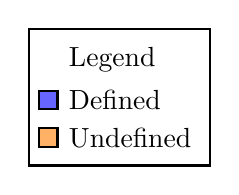
\begin{tikzpicture}
            \matrix [thick, draw=black] {
            \node[label=right:{Legend}] {}; \\
            \node[thick, shape=rectangle, draw=black, fill=blue!60,   label=right:{Defined}](0) {}; \\
            \node[thick, shape=rectangle, draw=black, fill=orange!60, label=right:{Undefined}](1) {}; \\
            };
        \end{tikzpicture}
    \end{subfigure}
    \caption{Breakdown of how many test approaches are undefined.}
    \label{fig:undefPies}
\end{figure*}

\fi

\subsection{Stopping Criteria}\label{stop-crit}

Unfortunately, we cannot continue looking for new approaches indefinitely. We
therefore need a ``stopping criteria'' to let us know when we are ``finished''
looking for test approaches in the literature. Our original plan was to iterate
steps \ref{step:ident-terms} and \ref{step:record-terms} until there are
diminishing returns, implying an approach of a complete taxonomy! However, due
to time constraints, this is infeasible, so our stopping point is artificially
imposed. With more time, we would find definitions for all terms we uncover as
described in \Cref{undef-terms}.

\ifnotpaper
    In addition to these undefined terms, some terms do not appear in
    the literature at all! While most test approaches arise as a result of our
    snowballing approach, we each have preexisting knowledge of what test
    approaches exist (a form of experience-based testing, if you will).
    As an example, we are surprised that property-based testing is not mentioned
    in any sources investigated, even considering it as a potential stopping point
    during our research%\thesisissueref{57,81,88,125}\qtodo{I think these issue
    % refs, along with some others may actually be worth keeping in our final
    % thesis/paper; thoughts?}
    . Test approaches such as these that arise independently of snowballing
    may serve as starting points for continued research if we do not find
    them in the literature using our iterative approach. The following terms come
    from previous knowledge, conversations with colleagues, research for other
    projects, or ad hoc cursory research to see what other test approaches exist:
    \newline

    \begin{minipage}{\textwidth}
        \begin{multicols}{2}
            \begin{enumerate}
                \item Chaos engineering
                \item Chosen-ciphertext \ifnotpaper\else \\ \fi attacks
                \item Concolic testing
                \item Concurrent testing
                \item Destructive testing
                \item Dogfooding
                \item Implementation-based testing
                \item Interaction-based \ifnotpaper\else \\ \fi testing
                      \ifnotpaper\else\columnbreak\fi
                \item Lunchtime attacks\ifnotpaper%
                          \footnote{In previous meetings, Dr.~Smith mentioned
                              that with the number of test approaches that suggest
                              that people just like to label everything as
                              ``testing'', he would not be surprised if something
                              like ``Monday morning testing'' existed. While
                              independently researching chosen-ciphertext attacks
                              out of curiosity, this prediction of a time-based
                              test approach came true with ``lunchtime attacks''.}
                      \fi
                \item Parallel testing
                \item Property-based testing
                \item Pseudo-random bit \ifnotpaper\else \\ \fi testing
                \item Rubber duck testing
                \item Scream testing
                \item Shadow testing
                \item Situational testing
            \end{enumerate}
        \end{multicols}
    \end{minipage}
\fi
